\documentclass{article}

\usepackage{graphicx}
\usepackage[utf8]{inputenc}
\usepackage[T1]{fontenc}
\usepackage[francais]{babel}
\usepackage{hyperref}
\usepackage{amsmath,amsfonts,amssymb}
\usepackage{Tkz-Tab}
\usepackage{wrapfig}
\usepackage{Verbatim}

\begin{document}

\title{L'algue tueuse
	\smallbreak
	TD n\degre3
	\smallbreak
	Modélisation mathématique
	\smallbreak
	Q4}
\author{Sibylle Roux \and Juliette Arazo \and Nicolas Le Gallo \and Tanguy Thomas}


\maketitle

\newpage

\tableofcontents

\newpage

\section{Etude du modèle logistique avec effet Allee et immigration}

\subsection{Etude numérique}

\subsubsection{Modèle avec variation de I}

\paragraph{Courbes de la vitesse d'accroissement}
\begin{center}
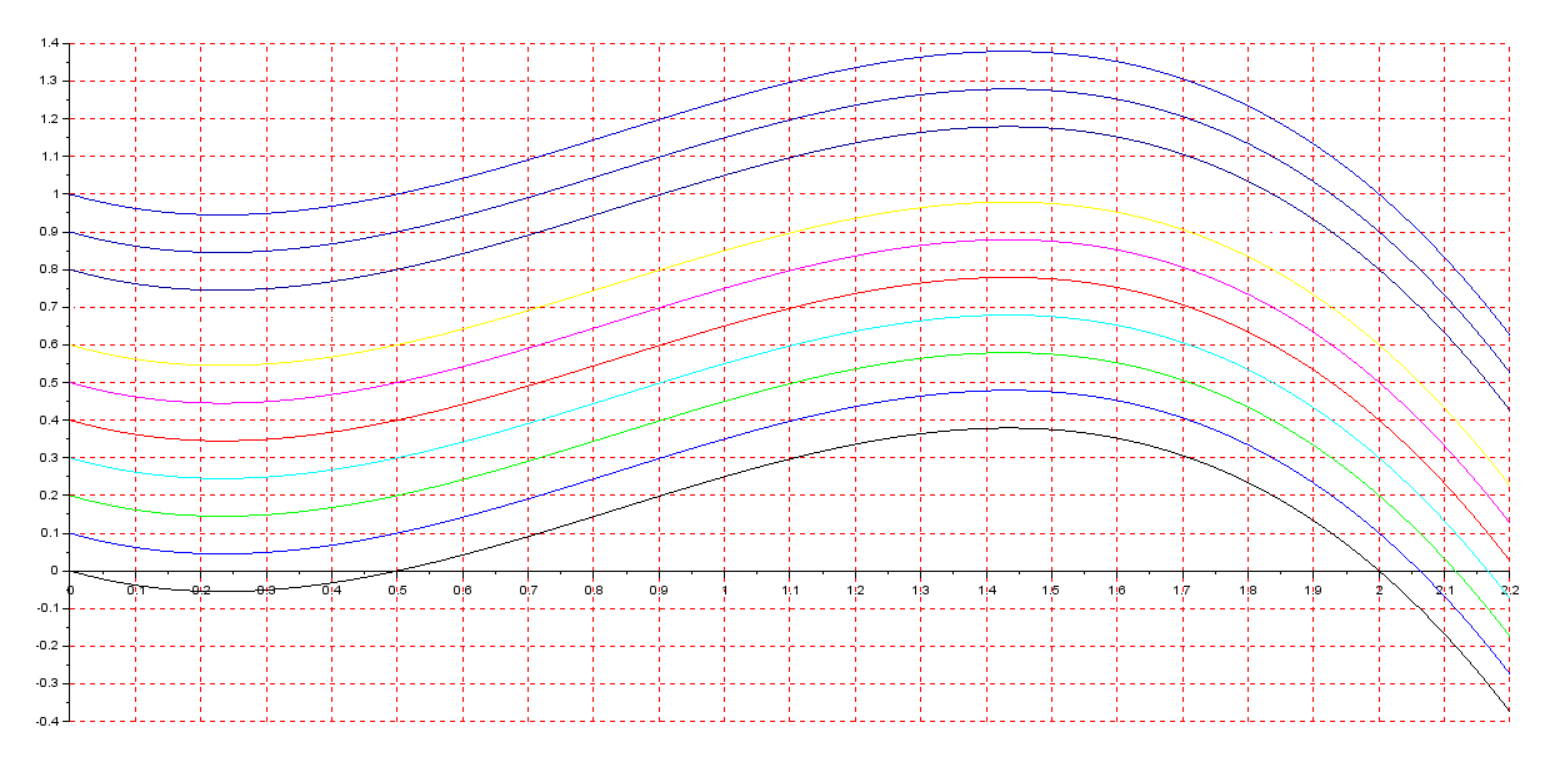
\includegraphics[width=300px]{img/part1/AlleeI.png}
\end{center}
Paramètres de modélisation : $K=2$  ; $r=0.5$ ; $A=0.5$ ; $I$ varie de 0 à 1 avec un pas de 0.1 
\paragraph{}
Sur ce graphique on peut voir les différentes courbes de la vitesse d'accroissement pour différentes valeurs de $I$. On peut voir que les variations de $I$ augmentent la vitesse d'acroissement de manière constante, cela influt donc aussi sur les points d'équilibres du modèle, en effet on voit bien que pour différentes valeurs de I, les points d'équilibres se déplacent sur la courbe, bien que les notions de stabilités/instabilités ne changent pas.
\paragraph{}
On remarque que avec un $I$ assez grand, l'effet Allee n'éteint plus la population mais ralentit seulement sa croissance. En effet 2 points d'équilibres peuvent disparaïtre à partir d'une valeur de I assez grande. Il ne reste donc plus qu'un seul point d'équilibre pour n'importe quelle valeur de population, il correspond à la capacité de charge du modèle (elle ne dépend plus que de $K$ mais aussi de $I$).
\newpage

\paragraph{Discrétisation du modèle}
\begin{center}
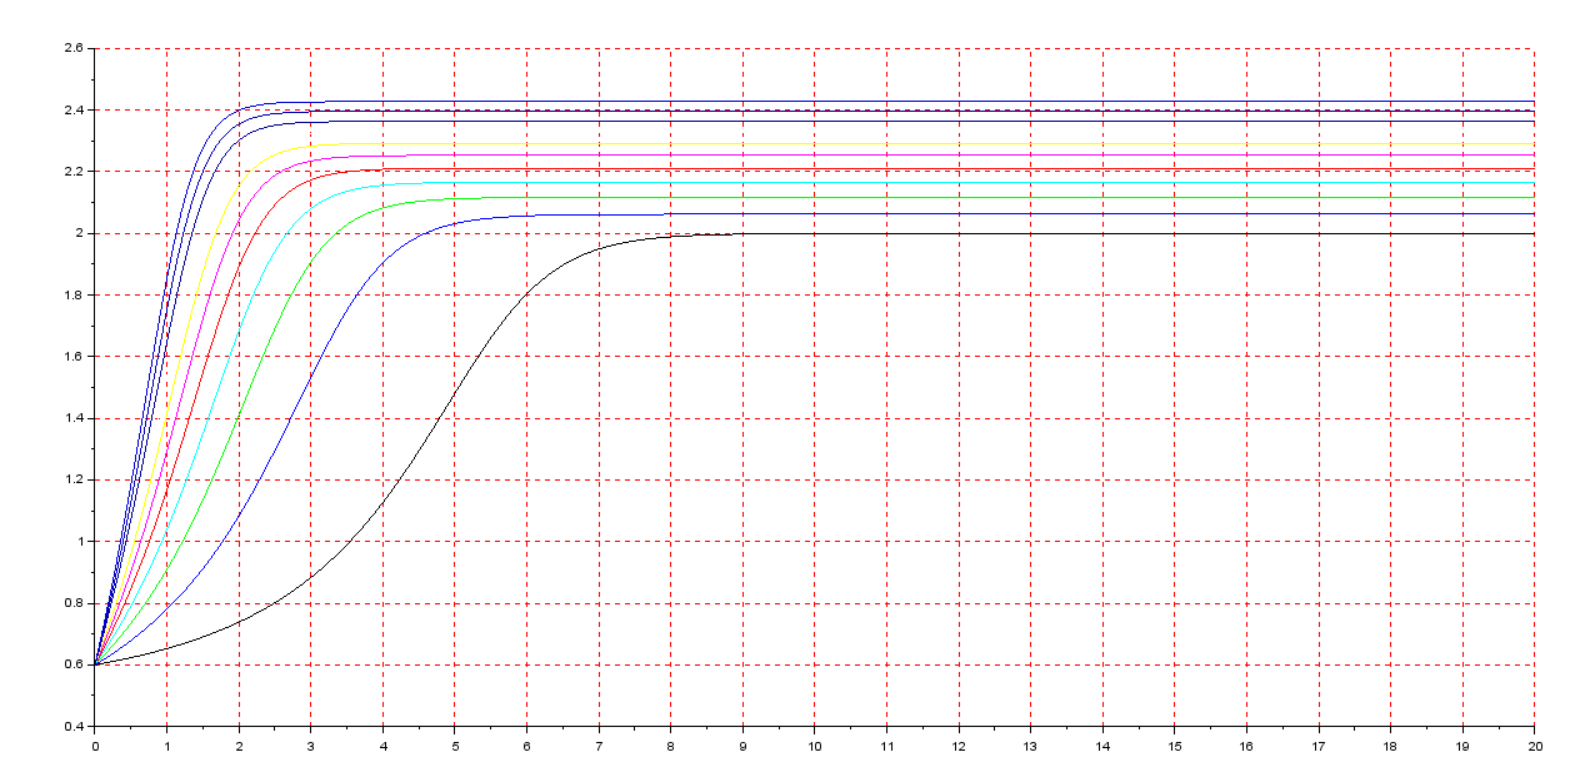
\includegraphics[width=300px]{img/part1/TrajI.png}
\end{center}
Paramètres de modélisation : $a=0.6$ ; $K=2$  ; $r=0.5$ ; $A=0.5$ ; $I$ varie de 0 à 1 avec un pas de 0.1
\paragraph{}
Sur ces courbes, on remarque bien que les variations de I, influent sur la capacité de charge du modèle, ainsi que la vitesse à laquelle il l'atteint.

\subsubsection{Modèle avec variation de K}

\paragraph{Courbes de la vitesse d'accroissement}
\begin{center}
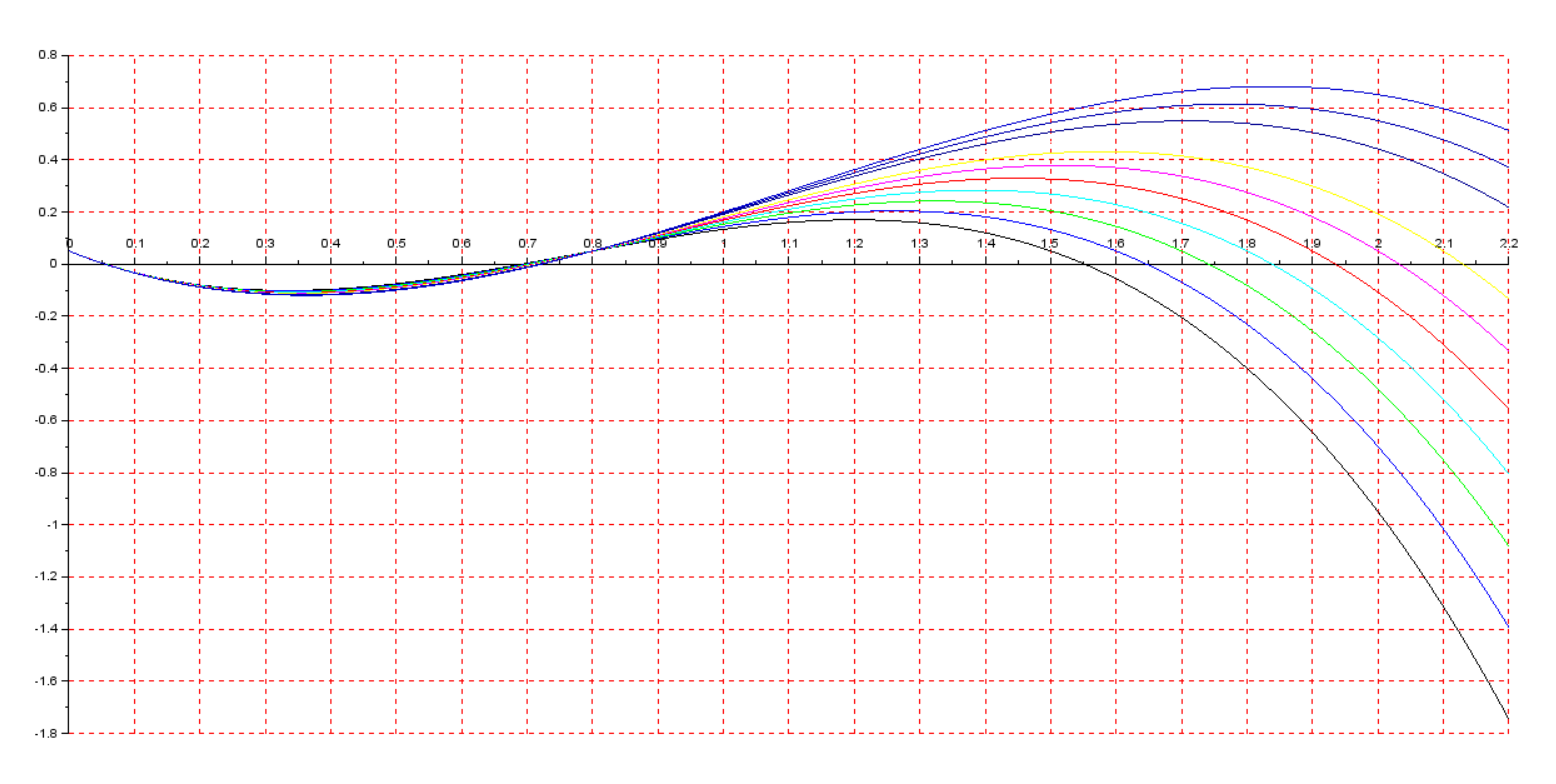
\includegraphics[width=300px]{img/part1/AlleeK.png}
\end{center}
Paramètres de modélisation : $r=1$ ; $A=0.8$ ; $I=0.05$ ; $K$ varie de 1.5 à 2.5 avec un pas de 0.1
\paragraph{}
Sur ce graphique on remarque que les variations de $K$ ont le même effet que sur le modèle logistique avec effet Allee. Les variations de $K$ déterminent la capacité de charge du modèle ($I$ influt aussi dans la capacité de charge). On remarque juste que le premier point d'équilibre stable (celui vers $0.05$, on l'appellera E1) permet à la population de ne jamais completement s'éteindre mais de tendre vers cette valeur.
On remarque donc que 2ème point d'équilibre (on l'appellera E2), celui instable vers $0.7$ est une valeur séparatrice des 2 bassins d'attractions :
\begin{itemize}
\item Lorsque la population initiale est inférieure à E2, la population va tendre vers l'équilibre stable E1,
\item Lorsque la population initiale est supérieure à E2, la population va tendre ves sa capacité de charge.
\end{itemize}

\paragraph{Discrétisation du modèle}
\begin{center}
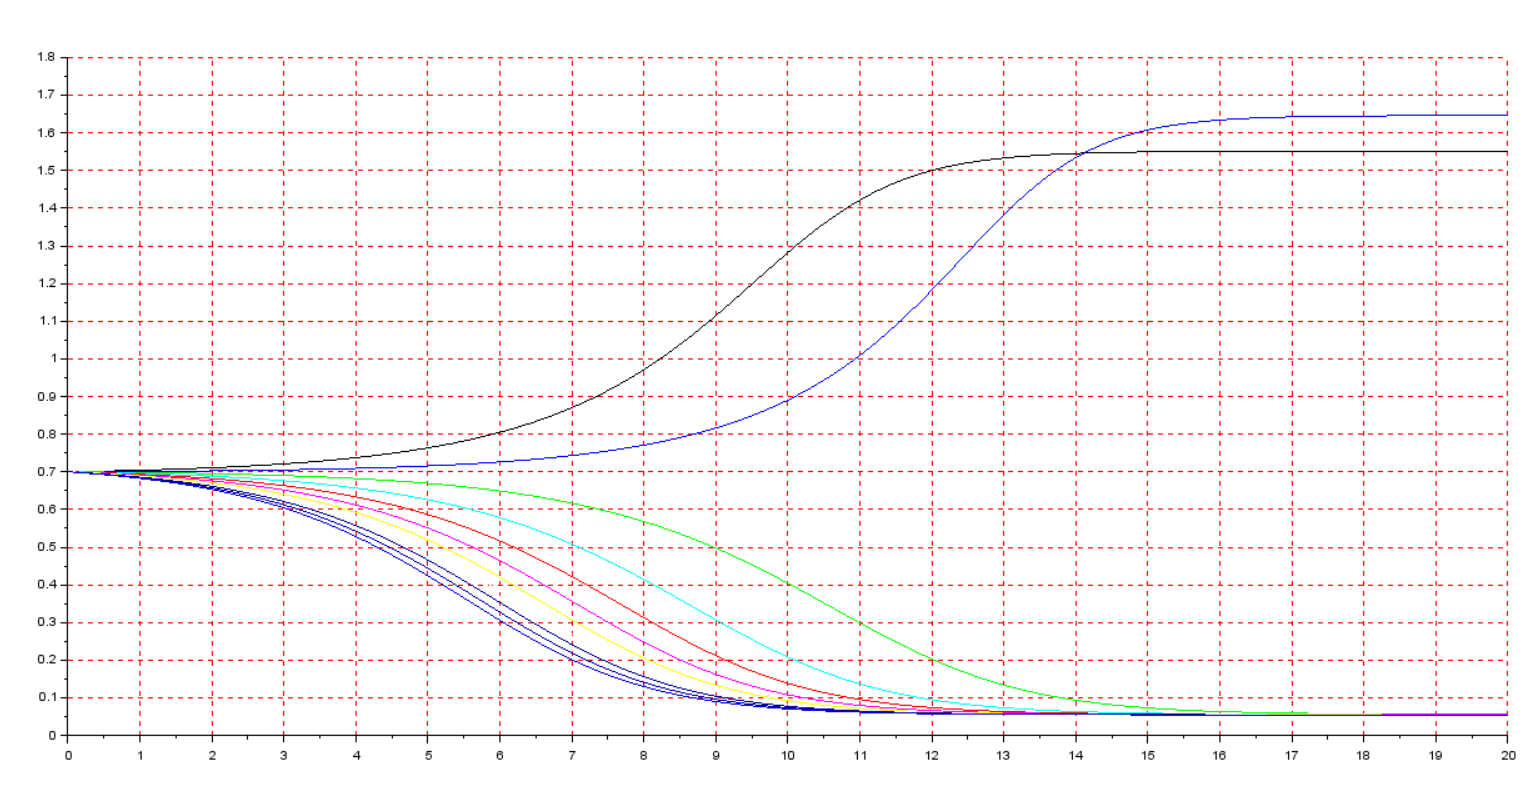
\includegraphics[width=300px]{img/part1/TrajK.png}
\end{center}
Paramètres de modélisation : $a=0.7$ ; $r=1$ ; $A=0.8$ ; $I=0.05$ ; $K$ varie de 1.5 à 2.5 avec un pas de 0.1
\paragraph{}

\subsubsection{Modèle avec variation de A}

\paragraph{Courbes de la vitesse d'accroissement}
\begin{center}
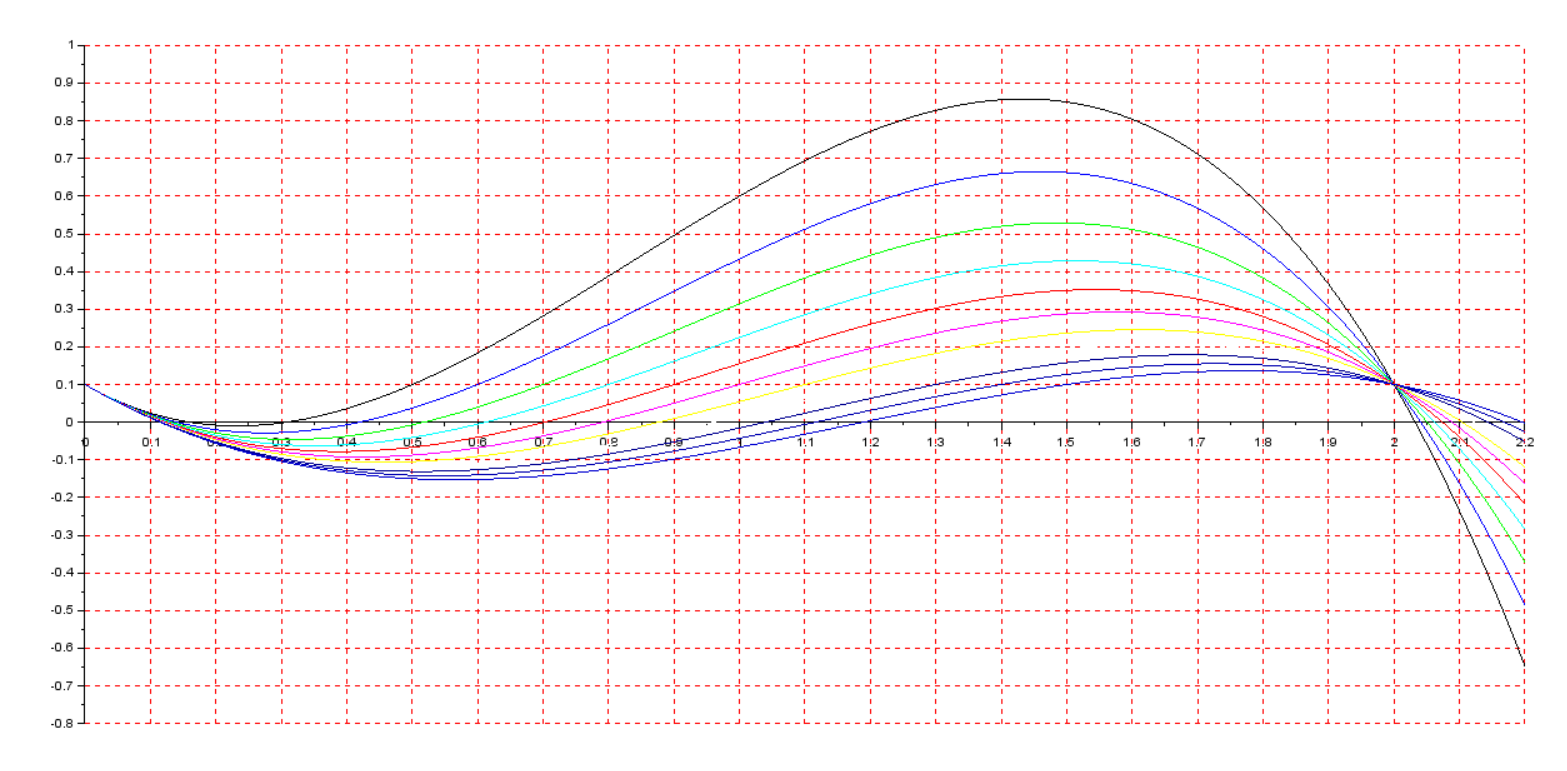
\includegraphics[width=300px]{img/part1/AlleeA.png}
\end{center}
Paramètres de modélisation : $I=0.1$ ; $K=2$ ; $r=1$  ; $A$ varie de 0.5 à 1.5 avec un pas de 0.1
\paragraph{}

\paragraph{Discrétisation du modèle}
\begin{center}
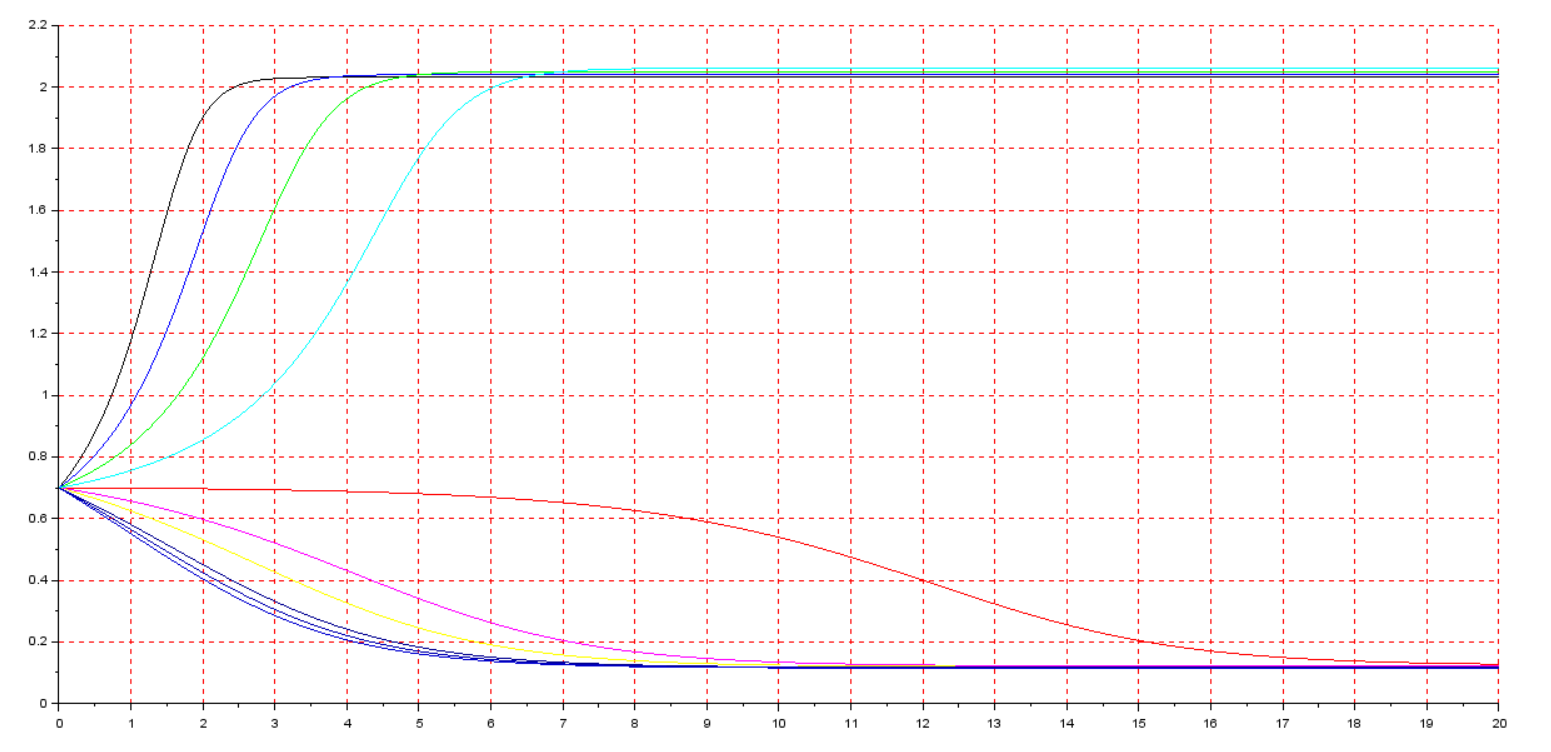
\includegraphics[width=300px]{img/part1/TrajA.png}
\end{center}
Paramètres de modélisation : $a=0.7$ ; $I=0.1$ ; $K=2$ ; $r=1$  ; $A$ varie de 0.5 à 1.5 avec un pas de 0.1
\paragraph{}

\subsubsection{Modèle avec variation de la population initiale}

\paragraph{Discretisation du modèle}
\begin{center}
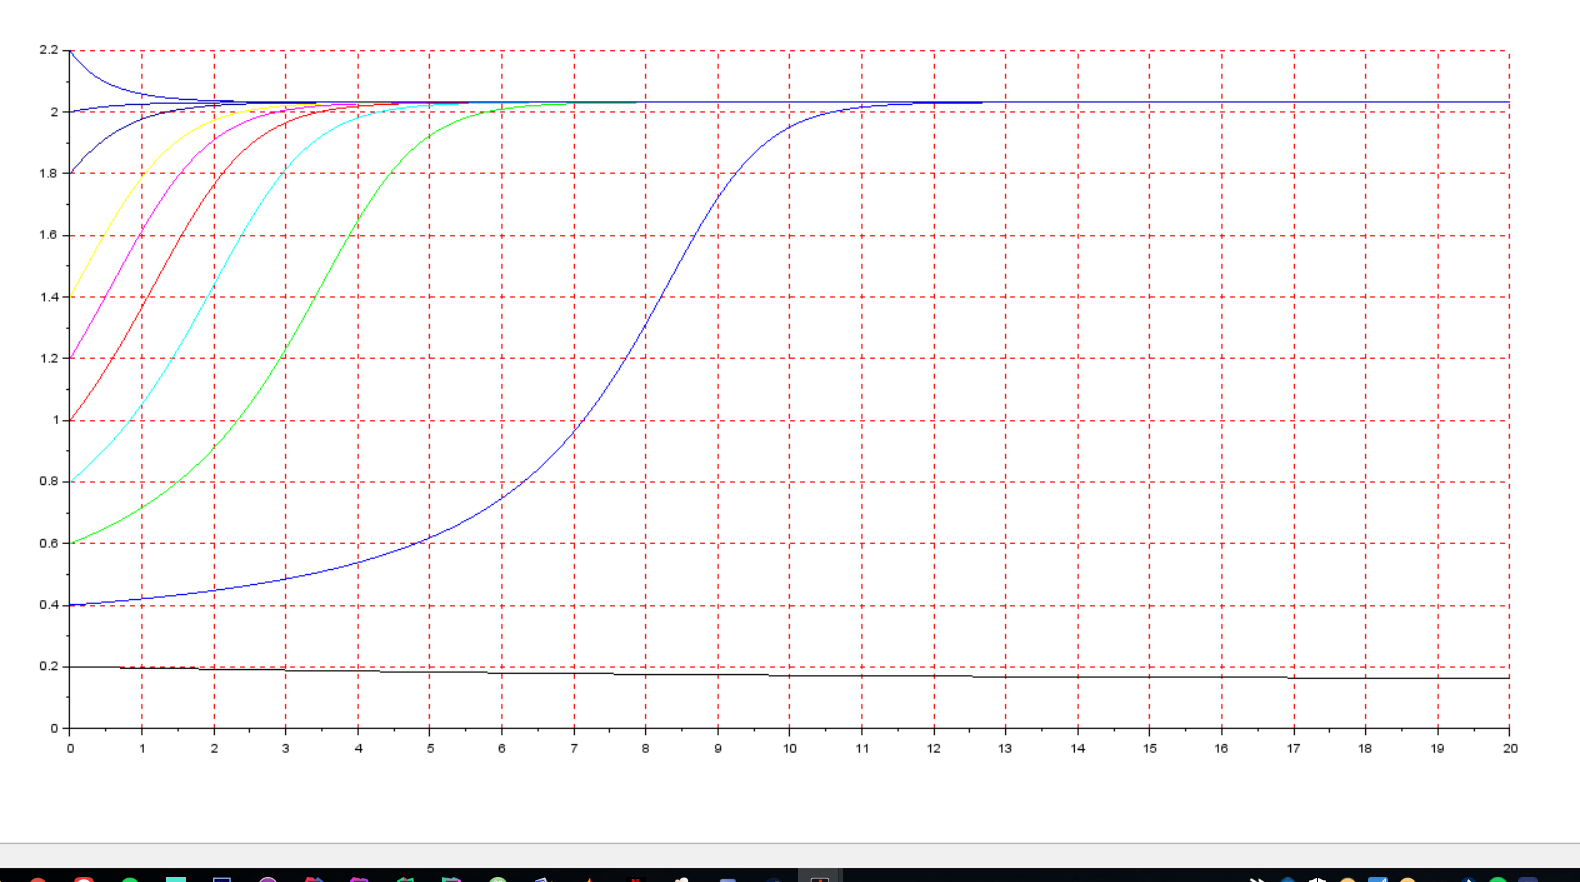
\includegraphics[width=300px]{img/part1/TrajPop.png}
\end{center}
Paramètres de modélisation : $A=0.5$ ; $I=0.1$ ; $K=2$ ; $r=0.5$  ; $a$ varie de 0.2 à 2.2 avec un pas de 0.2
\paragraph{}

\newpage

\subsection{Etude mathématique}


\subsection{Bilan}
\paragraph{}

\newpage
\section{Etude du modèle logistique avec prédation}

\subsection{Etude numérique}

\subsubsection{Modèle}

\paragraph{Vitesse d'accroissement}
\begin{center}
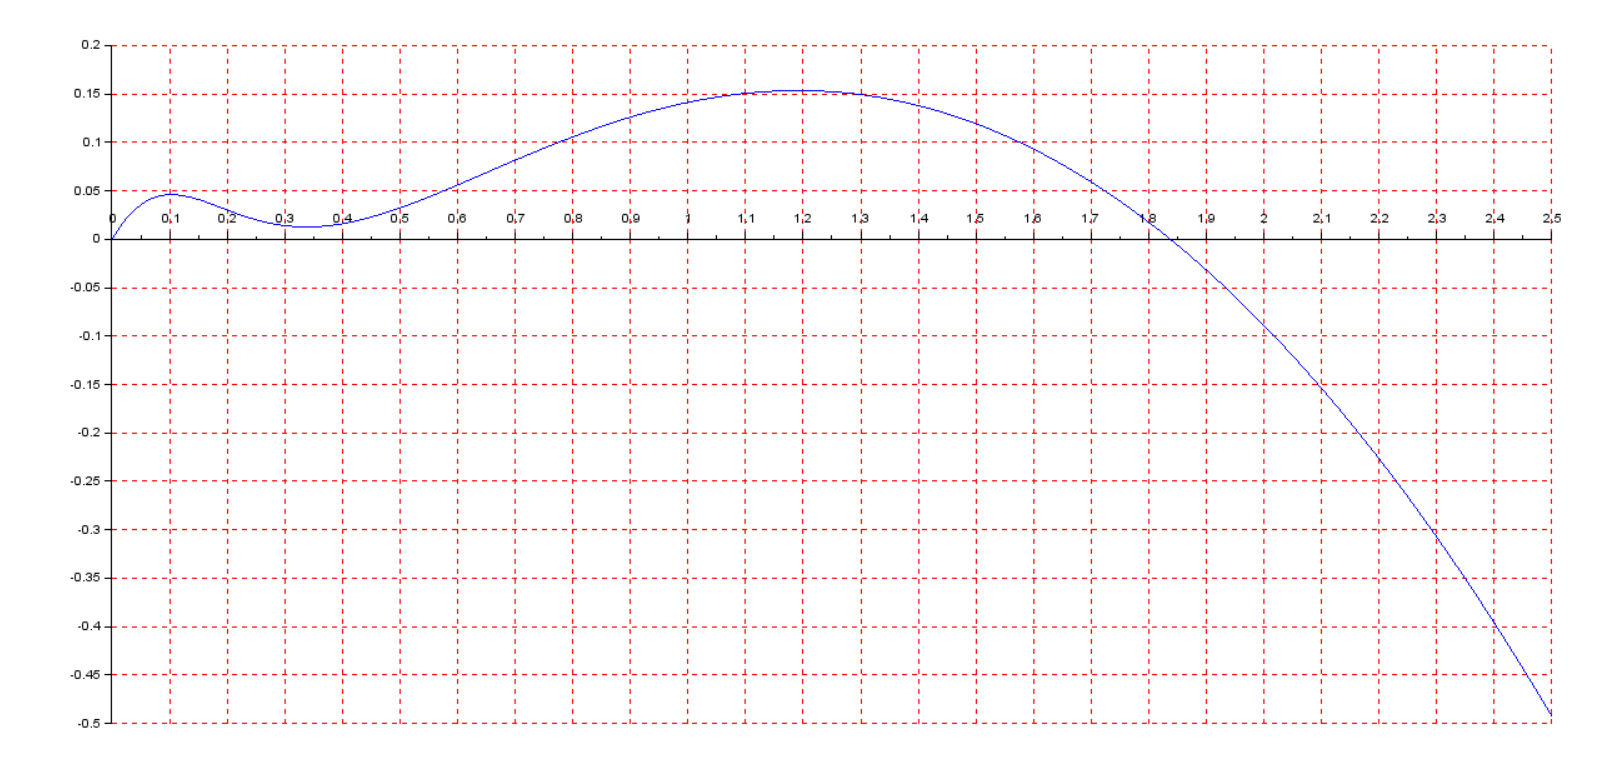
\includegraphics[width=300px]{img/part2/Log.png}
\end{center}
Paramètres de modélisation : $r=1$ ; $A=0.5$ ; $K=2.5$ ; $B=0.5$ ; $C=0.3$
\paragraph{}


\paragraph{Discretisation}
\begin{center}
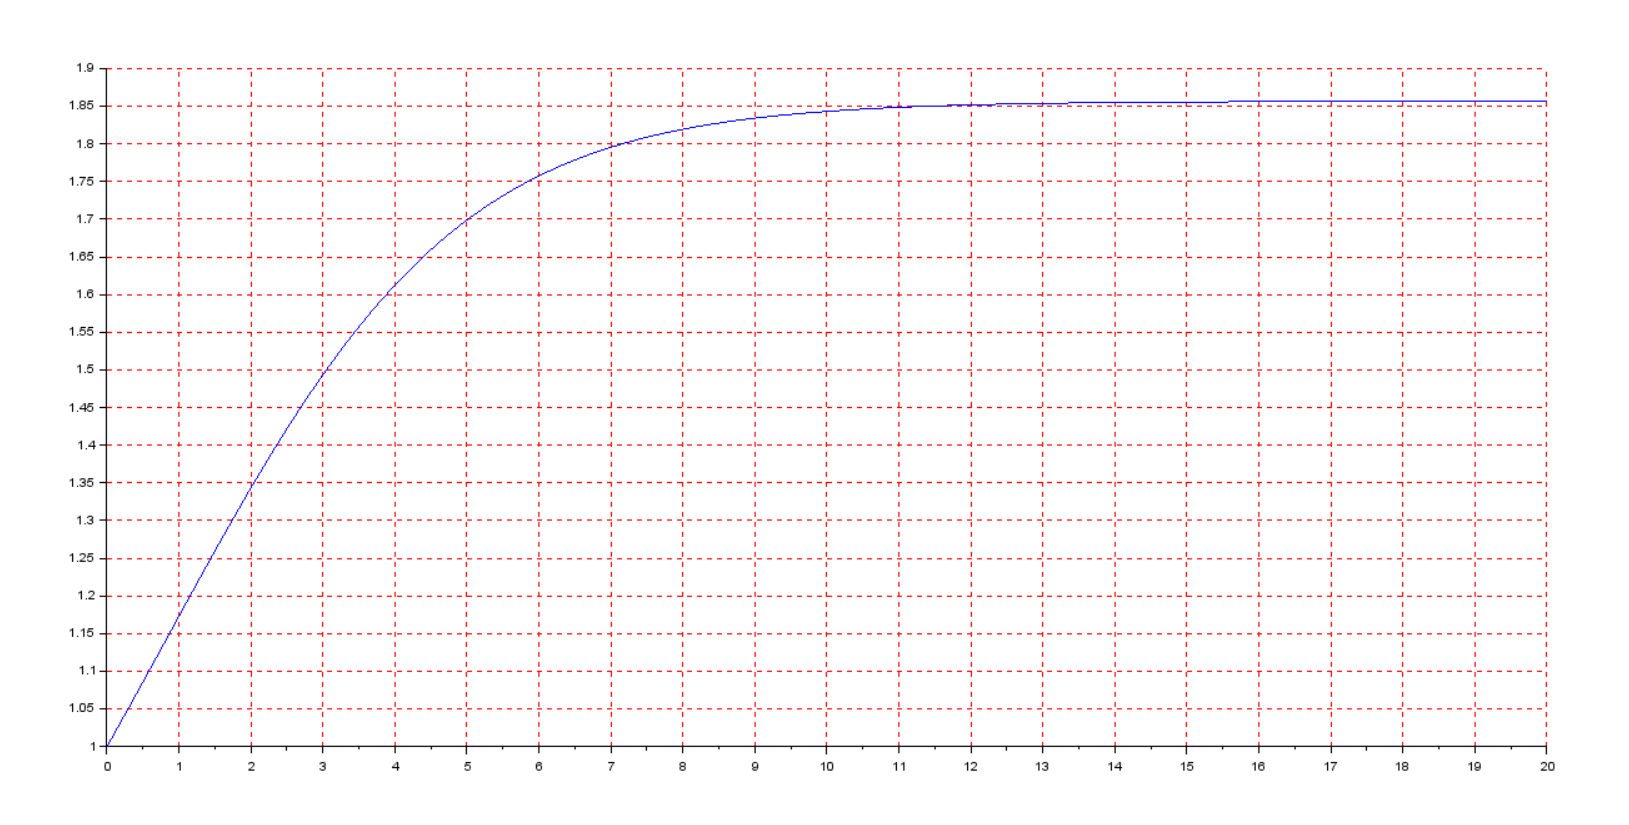
\includegraphics[width=300px]{img/part2/Traj.png}
\end{center}
Paramètres de modélisation : $r=1$ ; $A=0.5$ ; $K=2.5$ ; $B=0.5$ ; $C=0.4$ ; $h=0.05$ ; $a=1$
\paragraph{}

\subsubsection{Modèle avec variation de B}

\paragraph{Vitesse d'accroissement}
\begin{center}
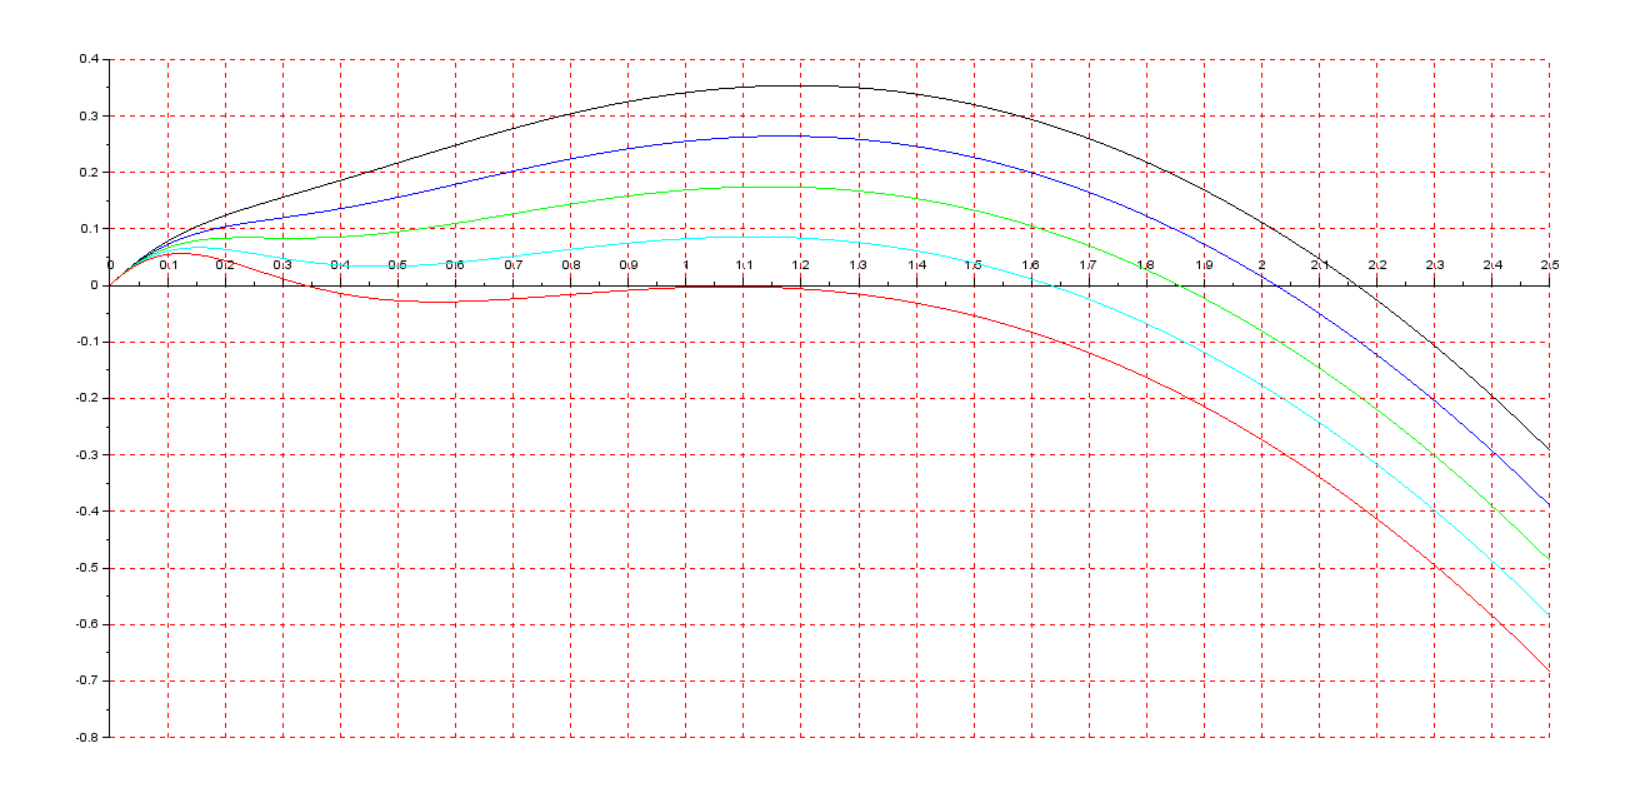
\includegraphics[width=300px]{img/part2/LogB.png}
\end{center}
Paramètres de modélisation : $r=1$ ; $A=0.5$ ; $K=2.5$ ; $C=0.4$ ; $B$ varie de 0.3 à 0.7 avec un pas de 0.1
\paragraph{}


\paragraph{Discretisation}
\begin{center}
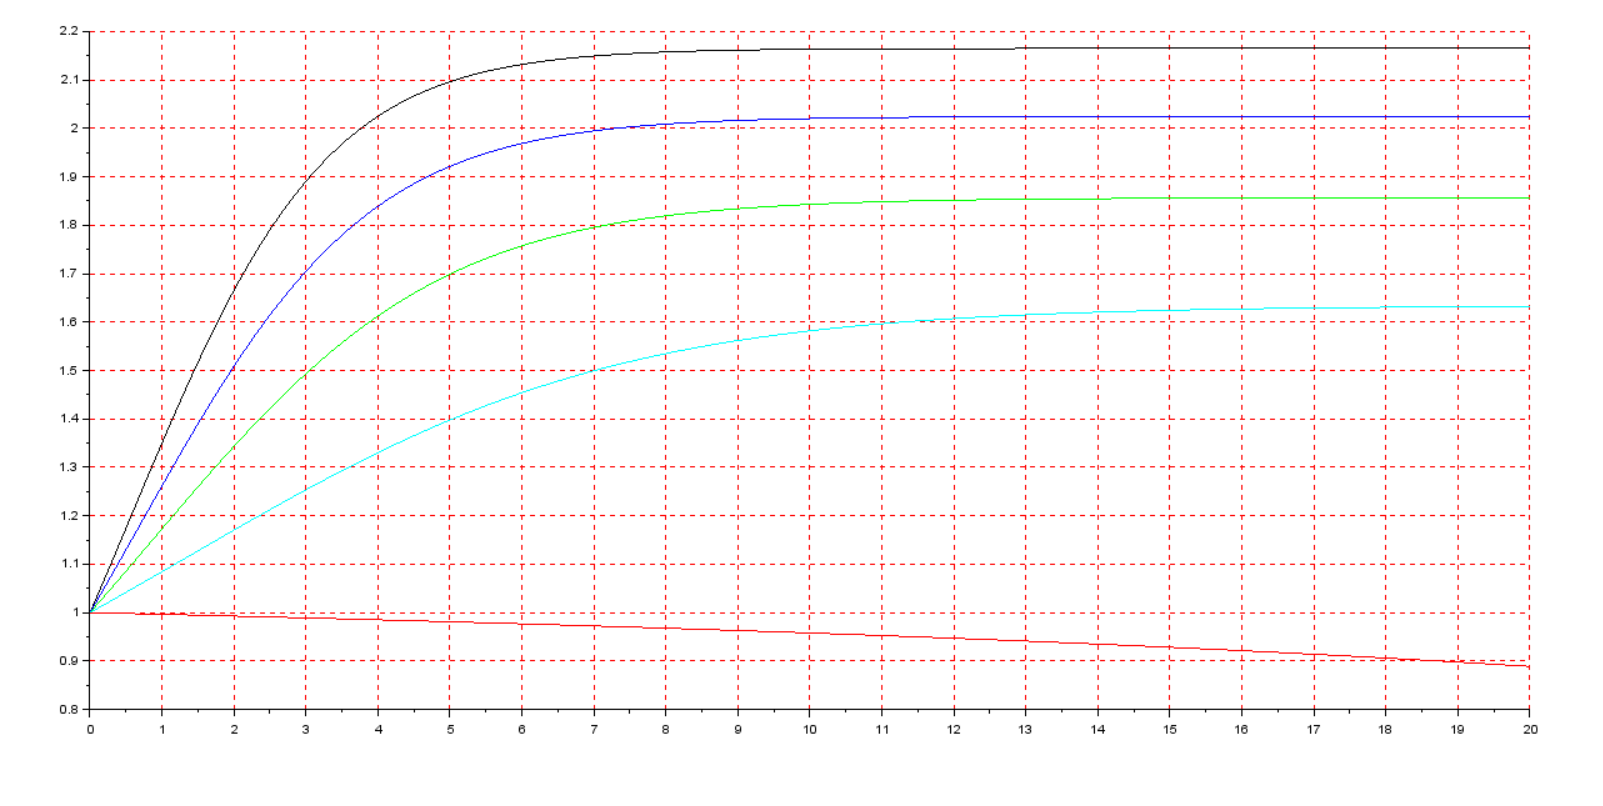
\includegraphics[width=300px]{img/part2/TrajB.png}
\end{center}
Paramètres de modélisation : $r=1$ ; $A=0.5$ ; $K=2.5$ ; $C=0.4$ ; $h=0.05$ ; $a=1$ ; $B$ varie de 0.3 à 0.7 avec un pas de 0.1
\paragraph{}

\subsubsection{Modèle avec variation de C}

\paragraph{Vitesse d'accroissement}
\begin{center}
\includegraphics[width=300px]{img/part2/logC.png}
\end{center}
Paramètres de modélisation :  $r=1$ ; $A=0.5$ ; $K=2.5$ ; $B=0.5$ ; $C$ varie de 0.2 à 0.4 avec un pas de 0.05
\paragraph{}


\paragraph{Discretisation}
\begin{center}
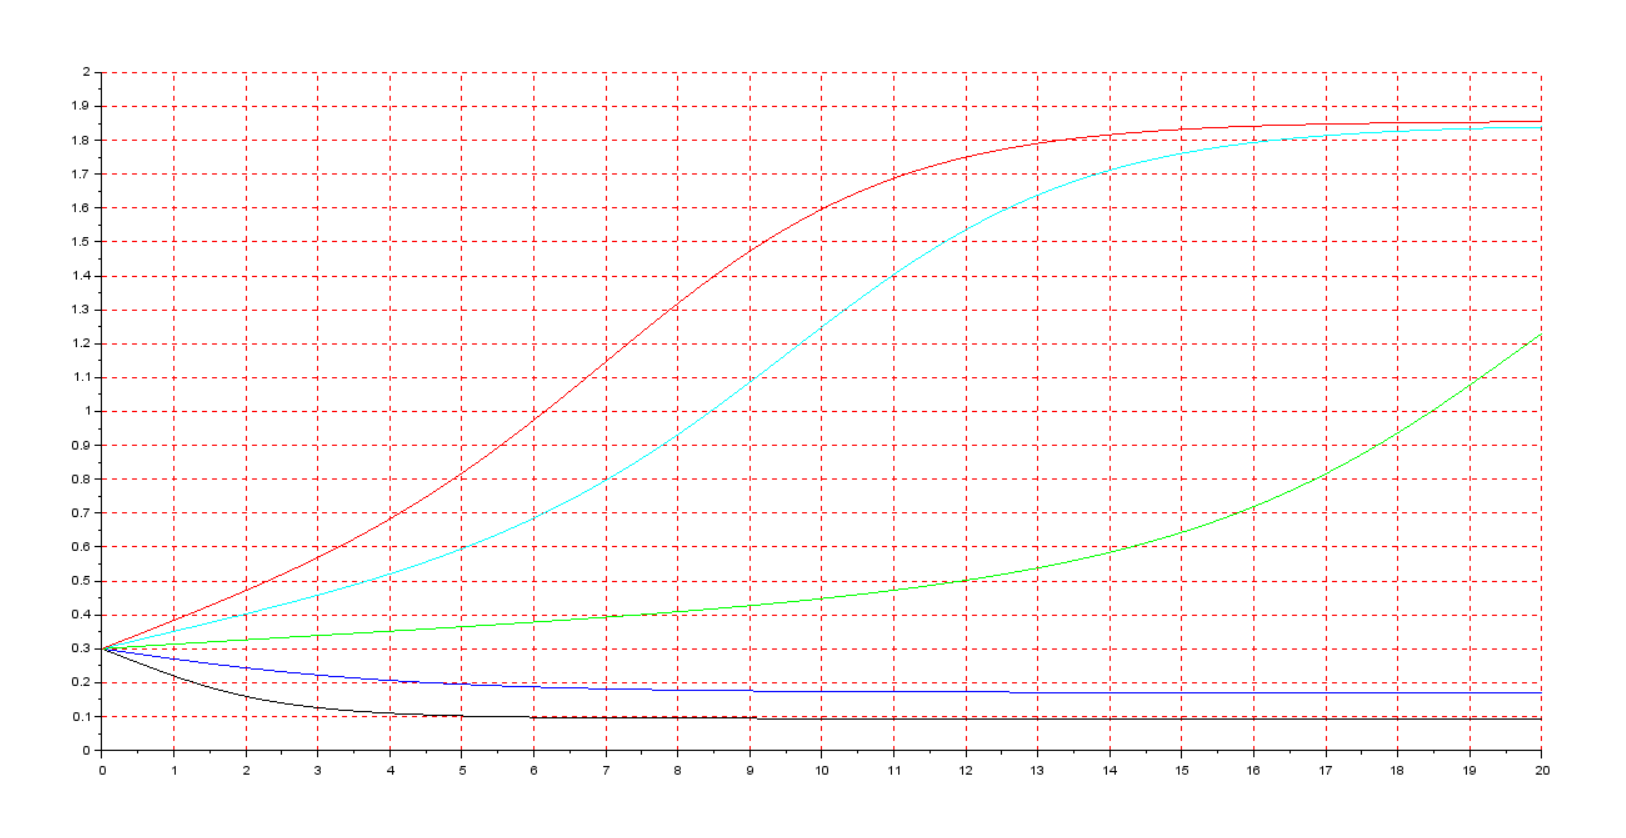
\includegraphics[width=300px]{img/part2/TrajC.png}
\end{center}
Paramètres de modélisation :  $r=1$ ; $A=0.5$ ; $K=2.5$ ; $B=0.5$ ; $h=0.05$ ; $a=0.3$ ; $C$ varie de 0.2 à 0.4 avec un pas de 0.05
\paragraph{}

\subsection{Etude mathématique}

\subsection{Bilan}
\paragraph{}


\newpage
\appendix

\section{Etude du modèle logistique avec effet Allee et immigration- Scripts Scilab}

\subsection{Modèle avec variation de I}

\subsubsection{Vitesse d'accroissement}

\begin{verbatim}
clear
clf

r = 0.5 ; A = 0.5 ; K = 2 ; // variables du modèles
Ivect=0:0.1:1; // variable qui varie
x = linspace(0, 2.2, 301); // vecteur contenant les valeurs de la vitesse d'accroissement

function f = allee_imig(x) // fonction qui calcule la vitesse d'accroissement
    f = r * x .* (x / A - 1 ) .* (1 - x / K)+ I // opérations vectorielles. x est un vecteur
endfunction

for i=1:11; // Bouclae qui va dessiner les différentes courbes
    I=Ivect(i); // Assignation valeur qui varie
    plot2d(x, allee_imig(x), style = i) // Tracé de la vitesse d'accroissement
end

// Définition des paramètres d'affichages
a=gca();
a.x_location = "origin";
a.grid=[5,5];
\end{verbatim}

\subsubsection{Discretisation}

\begin{verbatim}
clear
clf

Ivect=0:0.1:1; // variable qui varie
r = 0.5 ; A = 0.5 ; K = 2 ; h = 0.05 ; a = 0.6 ; // variables du modèles + pas de temps
ndate = 0:h:20; // vecteur des instants où on calcule la solution

function f = allee_img(x) // fonction qui calcule la vitesse d'accroissement
    f = r * x .* (x / A - 1 ) .* (1 - x / K)+I // opérations vectorielles. x est un vecteur
endfunction

x(1)=a; // Initialisation de la population initiale

for i=1:11; // Boucle qui va dessiner les différentes courbes
    I=Ivect(i); // Assignation valeur qui varie
    for n = 1:length(ndate) - 1 // Boucle qui calcule la courbe de la population
        x(n+1) = x(n) + h * allee_img(x(n)); // Calcul de la population
    end 
    plot2d(ndate, x, style = i) // Tracé de la discretisation
end

// Définition des paramètres d'affichages
a=gca();
a.x_location = "origin";
a.grid=[5,5];
\end{verbatim}

\subsection{Modèle avec variation de K}

\subsubsection{Vitesse d'accroissement}

\begin{verbatim}
clear
clf

r = 1 ; A = 0.8 ; I=0.05 ; // variables du modèles
Kvect=1.5:0.1:2.5; // variable qui varie
x = linspace(0, 2.2, 301); // vecteur contenant les valeurs de la vitesse d'accroissement

function f = allee_imig(x) // fonction qui calcule la vitesse d'accroissement
    f = r * x .* (x / A - 1 ) .* (1 - x / K)+ I // opérations vectorielles. x est un vecteur
endfunction

for i=1:11; // Boucle qui va dessiner les différentes courbes
    K=Kvect(i); // Assignation valeur qui varie
    plot2d(x, allee_imig(x), style = i) // Tracé de la vitesse d'accroissement
end

// Définition des paramètres d'affichages
a=gca();
a.x_location = "origin";
a.grid=[5,5];
\end{verbatim}

\subsubsection{Discretisation}

\begin{verbatim}
clear
clf

Kvect=1.5:0.1:2.5; // variable qui varie
r = 1 ; A = 0.8 ; I=0.05 ; h = 0.05 ; a = 0.7 ; // variables du modèles + pas de temps
ndate = 0:h:20; // vecteur des instants où on calcule la solution

function f = allee_img(x) // fonction qui calcule la vitesse d'accroissement
    f = r * x .* (x / A - 1 ) .* (1 - x / K)+I // opérations vectorielles. x est un vecteur
endfunction

x(1)=a; // Initialisation de la population initiale

for i=1:11; // Boucle qui va dessiner les différentes courbes
    K=Kvect(i); // Assignation valeur qui varie
    for n = 1:length(ndate) - 1 // Boucle qui calcule la courbe de la population
        x(n+1) = x(n) + h * allee_img(x(n)); // Calcul de la population
    end 
    plot2d(ndate, x, style = i) // Tracé de la discretisation
end

// Définition des paramètres d'affichages
a=gca();
a.x_location = "origin";
a.grid=[5,5];
\end{verbatim}

\subsection{Modèle avec variation de A}

\subsubsection{Vitesse d'accroissement}

\begin{verbatim}
clear
clf

r = 1 ; K = 2 ; I=0.1 ; // variables du modèles
Avect=0.5:0.1:1.5; // variable qui varie
x = linspace(0, 2.2, 301); // vecteur contenant les valeurs de la vitesse d'accroissement

function f = allee_imig(x) // fonction qui calcule la vitesse d'accroissement
    f = r * x .* (x / A - 1 ) .* (1 - x / K)+ I // opérations vectorielles. x est un vecteur
endfunction

for i=1:11; // Boucle qui va dessiner les différentes courbes
    A=Avect(i); // Assignation valeur qui varie
    plot2d(x, allee_imig(x), style = i) // Tracé de la vitesse d'accroissement
end

// Définition des paramètres d'affichages
a=gca();
a.x_location = "origin";
a.grid=[5,5];
\end{verbatim}

\subsubsection{Discretisation}

\begin{verbatim}
clear
clf

Avect=0.5:0.1:1.5; // variable qui varie
r = 1 ; K = 2 ; I=0.1 ; h = 0.05 ; a = 0.7 ; // variables du modèles + pas de temps
ndate = 0:h:20; // vecteur des instants où on calcule la solution

function f = allee_img(x) // fonction qui calcule la vitesse d'accroissement
    f = r * x .* (x / A - 1 ) .* (1 - x / K)+I // opérations vectorielles. x est un vecteur
endfunction

x(1)=a; // Initialisation de la population initiale

for i=1:11; // Boucle qui va dessiner les différentes courbes
    A=Avect(i); // Assignation valeur qui varie
    for n = 1:length(ndate) - 1 // Boucle qui calcule la courbe de la population
        x(n+1) = x(n) + h * allee_img(x(n)); // Calcul de la population
    end 
    plot2d(ndate, x, style = i) // Tracé de la discretisation
end

// Définition des paramètres d'affichages
a=gca();
a.x_location = "origin";
a.grid=[5,5];
\end{verbatim}

\subsection{Modèle avec variation de la population initiale}

\begin{verbatim}
clear
clf

avect=0.2:0.2:2.2; // variable qui varie
r = 0.5 ; K = 2 ; I=0.05 ; A = 0.5 ; h = 0.05 ; // variables du modèles + pas de temps
ndate = 0:h:20; // vecteur des instants où on calcule la solution

function f = allee_img(x) // fonction qui calcule la vitesse d'accroissement
    f = r * x .* (x / A - 1 ) .* (1 - x / K)+I // opérations vectorielles. x est un vecteur
endfunction

for i=1:11; // Boucle qui va dessiner les différentes courbes
    x(1)=avect(i); // Assignation valeur qui varie
    for n = 1:length(ndate) - 1 // Boucle qui calcule la courbe de la population
        x(n+1) = x(n) + h * allee_img(x(n)); // Calcul de la population
    end 
    plot2d(ndate, x, style = i) // Tracé de la discretisation
end

// Définition des paramètres d'affichages
a=gca();
a.x_location = "origin";
a.grid=[5,5];
\end{verbatim}

\section{Etude du modèle logistique avec prédation - Scripts Scilab}

\subsection{Modèle}

\subsubsection{Vitesse d'accroissement}

\begin{verbatim}
clear
clf

// variables du modèles
r = 1 ; A = 0.5 ; K = 2.5 ; B=0.5 ; C=0.3 ;
x = linspace(0, 2.5, 301);

function f = predation(x) // fonction qui calcule la vitesse d'accroissement
    f =r * x .* (1 - x / K) - B * (x.^2 ./ (x.^2 + C^2)) // opération vectorielle
endfunction

plot2d(x, predation(x), style = 2); // Tracé de la vitesse d'accroissement

// Définition des paramètres d'affichages
a=gca();
a.x_location = "origin";
a.grid=[5,5];
\end{verbatim}

\subsubsection{Discretisation}

\begin{verbatim}
clear
clf

// variables du modèles
r = 1 ; A = 0.5 ; K = 2.5 ; B=0.5 ; C=0.4 ; h = 0.05 ; a = 1;
ndate = 0:h:20; // vecteur des instants

function f = predation(x) // fonction qui calcule la vitesse d'accroissement
    f =r * x .* (1 - x / K) - B * (x.^2 ./ (x.^2 + C^2)) // opération vectorielle
endfunction

x(1) = a; // Initialisation de la population initiale

for n = 1:length(ndate) - 1 // Boucle qui calcule la courbe de la population
    x(n+1) = x(n) + h * predation(x(n)); // Calcul de la population
end

plot2d(ndate, x, style = 2) // Tracé de la trajectoire

// Définition des paramètres d'affichages
a=gca();
a.x_location = "origin";
a.grid=[5,5];
\end{verbatim}

\subsection{Modèle avec variation de B}

\subsubsection{Vitesse d'accroissement}

\begin{verbatim}
clear
clf

// variables du modèles
r = 1 ; A = 0.5 ; K = 2.5 ; C=0.4 ;
Bvect = 0.3:0.1:0.7; // variable qui varie
x = linspace(0, 2.5, 301);

function f = predation(x) // fonction qui calcule la vitesse d'accroissement
    f =r * x .* (1 - x / K) - B * (x.^2 ./ (x.^2 + C^2)) // opération vectorielle
endfunction

for i=1:5 // Boucle qui va dessiner les différentes courbes

    B=Bvect(i); // Assignation valeur qui varie

    plot2d(x, predation(x), style = i); // Tracé de la vitesse d'accroissement

end

// Définition des paramètres d'affichages
a=gca();
a.x_location = "origin";
a.grid=[5,5];
\end{verbatim}

\subsubsection{Discretisation}

\begin{verbatim}
clear
clf

Bvect = 0.3:0.1:0.7; // variable qui varie
// variables du modèles
r = 1 ; A = 0.5 ; K = 2.5 ; C=0.4 ; a = 1 ; h = 0.05 ;
ndate = 0:h:20; // vecteur des instants

function f = predation(x) // fonction qui calcule la vitesse d'accroissement
    f =r * x .* (1 - x / K) - B * (x.^2 ./ (x.^2 + C^2)) // opération vectorielle
endfunction

for i=1:5 // Boucle qui va dessiner les différentes courbes
    
    B=Bvect(i); // Assignation valeur qui varie
    x(1) = a; // Initialisation de la population initiale
    
    for n = 1:length(ndate) - 1 // Boucle qui calcule la courbe de la population
        x(n+1) = x(n) + h * predation(x(n)); // Calcul de la population
    end
    
    plot2d(ndate, x, style = i) // Tracé de la trajectoire

end

// Définition des paramètres d'affichages
a=gca();
a.x_location = "origin";
a.grid=[5,5];
\end{verbatim}


\subsection{Modèle avec variation de C}

\subsubsection{Vitesse d'accroissement}

\begin{verbatim}
clear
clf

// variables du modèles
r = 1 ; A = 0.5 ; K = 2.5 ; B=0.5 ;
Cvect = 0.2:0.05:0.4; // variable qui varie
x = linspace(0, 2.5, 301);

function f = predation(x) // fonction qui calcule la vitesse d'accroissement
    f =r * x .* (1 - x / K) - B * (x.^2 ./ (x.^2 + C^2)) // opération vectorielle
endfunction

for i=1:5 // Boucle qui va dessiner les différentes courbes
 
    C=Cvect(i); // Assignation valeur qui varie

    plot2d(x, predation(x), style = i); // Tracé de la vitesse d'accroissement

end

// Définition des paramètres d'affichages
a=gca();
a.x_location = "origin";
a.grid=[5,5];
\end{verbatim}

\subsubsection{Discretisation}

\begin{verbatim}
clear
clf

Cvect = 0.2:0.05:0.4; // variable qui varie
// variables du modèles
r = 1 ; A = 0.5 ; K = 2.5 ; B=0.5 ; h = 0.05 ; a = 0.3 ;
ndate = 0:h:20; // vecteur des instants

function f = predation(x) // fonction qui calcule la vitesse d'accroissement
    f =r * x .* (1 - x / K) - B * (x.^2 ./ (x.^2 + C^2)) // opération vectorielle
endfunction

for i=1:5 // Boucle qui va dessiner les différentes courbes
    
    C=Cvect(i); // Assignation valeur qui varie
    x(1) = a; // Initialisation de la population initiale
    
    for n = 1:length(ndate) - 1 // Boucle qui calcule la courbe de la population
        x(n+1) = x(n) + h * predation(x(n)); // Calcul de la population
    end
    
    plot2d(ndate, x, style = i) // Tracé de la trajectoire

end

// Définition des paramètres d'affichages
a=gca();
a.x_location = "origin";
a.grid=[5,5];
\end{verbatim}



\end{document}